\documentclass[tikz]{standalone}

\usetikzlibrary{positioning}

\begin{document}
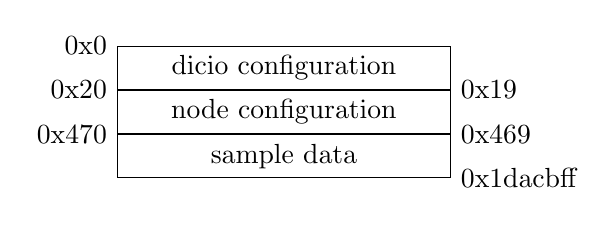
\begin{tikzpicture}
\begin{scope}[every node/.style={text width=4cm,align=center}]
  \node[draw] (dicio) {dicio configuration};
  \node[draw,below=0cm of dicio] (nodeconfig) {node configuration};
  \node[draw,below=0cm of nodeconfig] (data) {sample data};
\end{scope}
  
  \draw (dicio.north west) node[anchor=east] {0x0};
  \draw (nodeconfig.north west) node[anchor=east] {0x20};
  \draw (data.north west) node[anchor=east] {0x470};
  
  \draw (dicio.south east) node[anchor=west] {0x19};
  \draw (nodeconfig.south east) node[anchor=west] {0x469};
  \draw (data.south east) node[anchor=west] {0x1dacbff};
\end{tikzpicture}

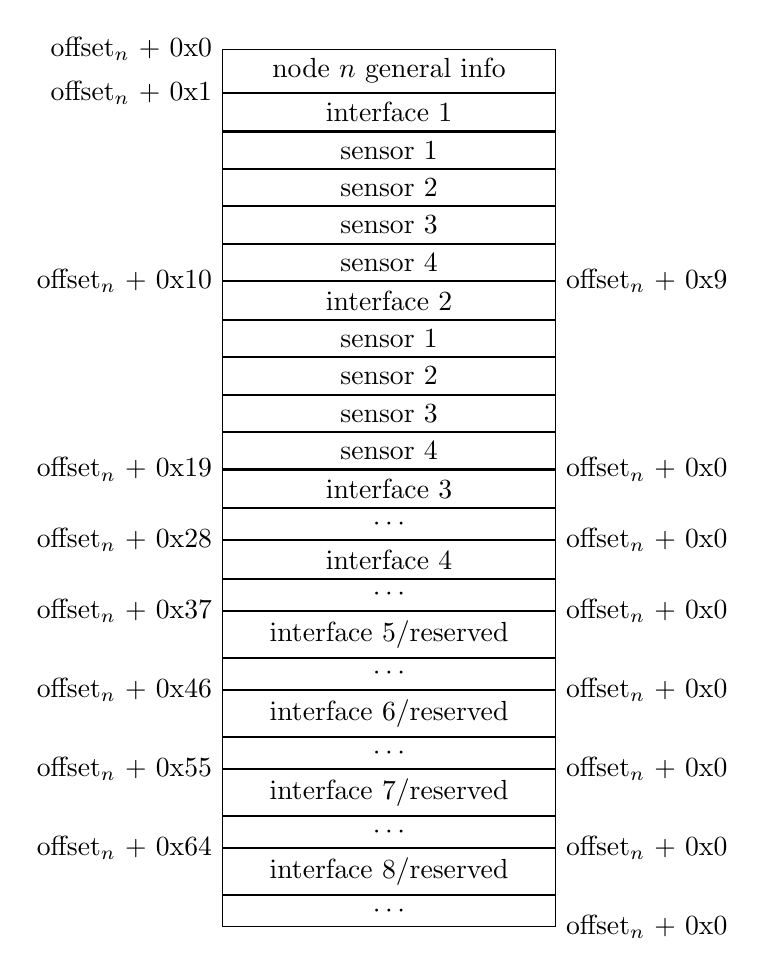
\begin{tikzpicture}
\begin{scope}[every node/.style={text width=4cm,align=center}]
  \node[draw] (info) {node $n$ general info};
  \node[draw,below=0cm of info] (if1) {interface 1};
  \node[draw,below=0cm of if1] (s1-1) {sensor 1};
  \node[draw,below=0cm of s1-1] (s1-2) {sensor 2};
  \node[draw,below=0cm of s1-2] (s1-3) {sensor 3};
  \node[draw,below=0cm of s1-3] (s1-4) {sensor 4};
  \node[draw,below=0cm of s1-4] (if2) {interface 2};
  \node[draw,below=0cm of if2] (s2-1) {sensor 1};
  \node[draw,below=0cm of s2-1] (s2-2) {sensor 2};
  \node[draw,below=0cm of s2-2] (s2-3) {sensor 3};
  \node[draw,below=0cm of s2-3] (s2-4) {sensor 4};
  \node[draw,below=0cm of s2-4] (if3) {interface 3};
  \node[draw,below=0cm of if3] (if3-dots) {$\cdots$};
  \node[draw,below=0cm of if3-dots] (if4) {interface 4};
  \node[draw,below=0cm of if4] (if4-dots) {$\cdots$};
  \node[draw,below=0cm of if4-dots] (if5) {interface 5/reserved};
  \node[draw,below=0cm of if5] (if5-dots) {$\cdots$};
  \node[draw,below=0cm of if5-dots] (if6) {interface 6/reserved};
  \node[draw,below=0cm of if6] (if6-dots) {$\cdots$};
  \node[draw,below=0cm of if6-dots] (if7) {interface 7/reserved};
  \node[draw,below=0cm of if7] (if7-dots) {$\cdots$};
  \node[draw,below=0cm of if7-dots] (if8) {interface 8/reserved};
  \node[draw,below=0cm of if8] (if8-dots) {$\cdots$};
\end{scope}
  
  \draw (info.north west) node[anchor=east] {offset$_n$ + 0x0};
  \foreach \x/\y in {1/1,2/10,3/19,4/28,5/37,6/46,7/55,8/64} {
    \draw (if\x.north west) node[anchor=east] {offset$_n$ + 0x\y};
  }
  \foreach \x/\y in {1/9,2/0} {
    \draw (s\x-4.south east) node[anchor=west] {offset$_n$ + 0x\y};
  }
  \foreach \x/\y in {3/0,4/0,5/0,6/0,7/0,8/0} {
    \draw (if\x-dots.south east) node[anchor=west] {offset$_n$ + 0x\y};
  }
  
\end{tikzpicture}
\end{document}